\section{Passivity-Based Control} \label{section:pssivity}
Initial presentation of passive-decomposition is found in D. Lee et. al 2004. \cite{passive-decomp-mechanical-coord-req}. It decomposes the overall dynamics into shape system addressing the coordination aspect, locked system representing internal dynamics wrt. the holonomic constraints and dynamic couplings between the locked and shape systems.The coupled dynamics can be canceled out without violating passivity. Thus, the coordination aspect (shape system) and the dynamics of the coordinated (locked) system can be decoupled from each other while enforcing passivity. By designing the locked and shape controls to enforce passivity  of their respective systems, the closed-loop system energetic passivity is guaranteed. A brief introduction towards passive-decomposition is given as follows. \\
Consider a group of $m$-mechanical systems such that the $i$-th agent's dynamics evolve on a configuration manifold $\Ma_i$:
	\begin{equation}
	M_i(\textbf{q}_i)\nabla^i_{\textbf{v}_i} \textbf{v}_i = \textbf{T}_i + \textbf{F}_i, \;\;\; i = 1,...,m,
\end{equation}
where the following terms are defined as follows:
\begin{itemize}
	\item $\textbf{T}_i, \textbf{F}_i\in\text{T}_{\textbf{q}_i}^*\Ma_i$ - control and environmental force covectors that exist in a cotangent manifold at point $\textbf{q}_i$
	
	\item $\textbf{v}_i \in \text{T}_i^{*}\Ma_i$ - system velocity at point $\textbf{q}_i$ in the tangent manifold
	
	\item $\nabla^i_{\textbf{v}_i}$ - this symbol represents a covariant derivative operator, the Levi-Civita connection. It provides a well defined method of differentiating vector fields along the ${\textbf{v}_i}$ direction on the tangent bundle $\text{T}\Ma_i$.
	
	\item $M_i(\textbf{q}_i)$ - inertia tensor which maps vectors from tangent space to cotangent space at point $\textbf{q}$, defined as $M:\text{T}_{\textbf{q}}\Ma \mapsto \text{T}_{\textbf{q}}^*\Ma$
\end{itemize}

Furthermore, the supply rate for the m-agent mechanical system is defined as follows.
\begin{equation}
	s_\rho(\textbf{v}_i, \textbf{T}_i) = \langle\textbf{F}_i, \dot{\textbf{q}}_i \rangle + ... + \langle\textbf{F}_m, \dot{\textbf{q}}_m \rangle \, ,
\end{equation}
where $\langle \cdot, \cdot \rangle: \text{T}_{\textbf{q}}^*\Ma \times \text{T}_{\textbf{q}}\Ma  \rightarrow \mathbb{R}$. \\
\noindent For safe and stable interaction an energetic passivity condition where $\exists d\in\mathbb{R}$ such that: 
\begin{equation}
	 \int_{0}^{t}	s_\rho(\textbf{v}_i(\tau), \textbf{T}_i(\tau))d\tau \geq -d^2, \;\forall t\geq 0
\end{equation}
Similar condition is employed to induce controller passivity. \\
Introducing the coordination map $h:\Ma^n \rightarrow \Na^m$ which holds the holonomic constraints, at each point of the configuration manifold $q\in\Ma$, the corresponding tangent space $\text{T}_q\Ma$
is split into two orthogonal vector spaces as follows:
\begin{equation}
	\text{T}_q\Ma = \text{T}_q^\top \Ma \oplus \text{T}_q^{\perp} \Ma
\end{equation}
The tangential and perpendicular spaces are defined respectively:
\begin{gather}
	\text{T}_q^\top\Ma := span \{v \in \text{T}_q\Ma \, \vert \, h_*(v) = 0\}  \\
	\text{T}_q^\perp\Ma := span \{w \in \text{T}_q\Ma \, \vert \, \langle \langle v, w \rangle \rangle, \, \forall v \in \text{T}_q^\top \Ma  \}, 
\end{gather}
where $h_*: \text{T}_q\Ma \rightarrow \text{T}_{h(q)}\Na$ is the push-forward of the coordination map. \\
By applying the orthogonal decomposition to the model dynamics we are able to decouple the shape and locked dynamics, while applying a control law cancel the coupling which essentially sums up the notion of passive-decomposition.

A concrete application of the passive-decomposition concepts on a UAV system can be found in \cite{passive-decomp-quadrotor-with-robotic-manip}. The authors show that the Lagrange dynamics of quadrotor-manipulator systems can be completely decoupled into: the center-of-mass dynamics in E(3), which, similar to the standard quadrotor dynamics, is point-mass dynamics with under-actuation  and  gravity  effect; the  “internal rotational” dynamics  of  the  quadrotor’s  rotation  and  manipulator configuration, which assumes the form of standard Lagrange dynamics  of  robotic manipulator with full-actuation and nogravity effect.  
\begin{figure}[H]
	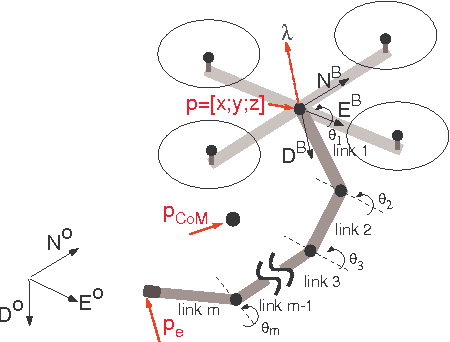
\includegraphics[width=0.95\columnwidth]{figure/aerial_manip.png}	
	\centering
	\caption{This $\text{figure}^{\cite{passive-decomp-quadrotor-with-robotic-manip}}$ represents a quadrotor UAV with a generalized m-DOF robot arm. The UAV platform's position is denoted with $\textbf{p}$, $\textbf{p}_e$ represents the end-effector position while $\textbf{p}_{CoM}$ is the center-of-mass vector of the entire quadrotor-manipulator system. It is worth nothing that a general case is considered where $\textbf{p}_{CoM} \neq\textbf{p}$.  }
	\label{fig:aerial_manip}
\end{figure}
\noindent A backstepping-like end-effector tracking control law is proposed, which allows  assignment of different roles for the center-of-mass control and internal rotational dynamics  control according to task objectives.

A similar passivity-based control design is presented in \cite{decoupled-aerial-manipulation} for quadrotor-manipulator UAV system utilizing a PID cascade  unlike the previously shown backstepping controller. Proposed control algorithms are implemented in the MATLAB/
Simulink environment and tested using the highly nonlinear system model in simulation. 
The controller robustness is checked by applying disturbance forces from different 
directions at the tip point of the 2-DOF robotic arm.

In \cite{passivity-backstepping}  a novel unified passivity-based adaptive backstepping control framework is proposed for ‘mixed’ quadrotor UAVs. Which consists of the translation dynamics with thrust force input and the attitude kinematics with the angular velocity input evolving on SE(3). Its application to haptic teleoperation over the Internet is also presented with dynamic-extension like filter to address discontinuous communication and a complete stability/collision-avoidance analysis is provided.

\cite{passivity-based-formation-load}
\cite{passive-variable-impedance-compliant} 
\cite{max-wrench-min-energy} 
\cite{quadrotor-itneraction-environment} 
\cite{passivity-based-payload-minimum-swing} 
\cite{passivity-based-crop} 
\cite{payload-and-human}
\cite{door-opening}
\cite{passivity-based-physical-interaction}